\documentclass[%
	11pt,
	a4paper,
	utf8,
	%twocolumn
		]{article}	

\usepackage{style_packages/podvoyskiy_article_extended}


\begin{document}
\title{Заметки по машинному обучению и анализу данных}

\author{\itshape Подвойский А.О.}

\date{}
\maketitle

\thispagestyle{fancy}

Здесь приводятся заметки по некоторым вопросам, касающимся машинного обучения, анализа данных, программирования на языках \texttt{Python}, \texttt{R} и прочим сопряженным вопросам так или иначе, затрагивающим работу с данными.

\tableofcontents

\section{Градиентный бустинг}

\subsection{Общие сведения}

\subsection{Особенности реализации в пакете \texttt{sklearn}}

\subsection{Особенности реализации в пакете \texttt{XGBoost}}

\subsubsection{Установка пакета \texttt{xgboost} на \texttt{Windows}}

Устанавливать пакет \texttt{xgboost} рекомендуется с помощью следующей команды

\begin{lstlisting}[
numbers = none
]
conda install -c anaconda py-xgboost 
\end{lstlisting}

Существует альтернативный способ установки пакета \texttt{xgboost} (разумеется он работает и для других пакетов). Для начала требуется вывести список доступных каналов (см. \pic{fig:xgboost_conda_search}), по которым будет проводиться поиск интересующего пакета (в данном случае пакета \texttt{xgboost}), а затем можно воспользоваться конструкцией

\begin{lstlisting}[
numbers = none
]
anaconda search -t conda xgboost
\end{lstlisting}

\begin{figure}[h]
	\centering
	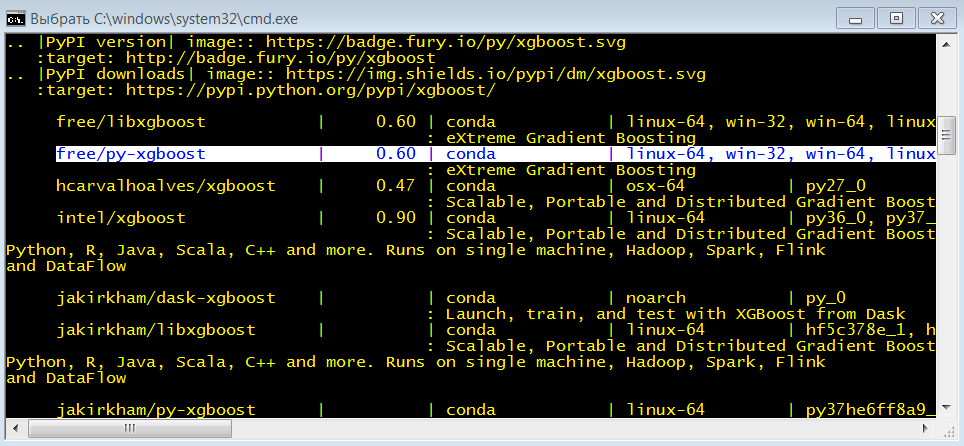
\includegraphics[scale=0.85]{figures/xgboost_conda_search.png}
	\caption{Окно командной оболочки \texttt{cmd.exe} со списком доступных каналов, по которым будет проводиться поиск пакета \texttt{xgboost} }\label{fig:xgboost_conda_search}
\end{figure}


После, выбрав канал, можно приступать к установке пакета

\begin{lstlisting}[
numbers = none
]
conda install -c free py-xgboost
\end{lstlisting}

\subsubsection{Простой пример работы с \texttt{xgboost} и \texttt{shap}}

Решается задача бинарной классификации. Требуется построить модель, предсказывающую годовой доход заявителя по порогу \$50'000 (то есть больше или меньше \$50'000 зарабатывает заявитель в год). Используется набор данных  UCI Adult income

\begin{lstlisting}[
style = ironpython,
numbers = none
]
import xgboost
import shap  # для оценки важности признаков вычисляются значения Шепли (Shapley value)
import numpy as np
import matplotlib.pyplot as plt
from sklearn.model_selection import train_test_split

shap.initjs()

X, y = shap.datasets.adult()
X_display, y_display = shap.datasets.adult(display=True)

X_train, X_test, y_train, y_test = train_test_split(X, y, test_size=0.2, random_state=7)
d_train = xgboost.DMatrix(X_train, label=y_train)
d_test = xgboost.DMatrix(X_test, label=y_test)

params = {
    'eta' : 0.01,
    'objective' : 'binary:logistic',
    'subsample' : 0.5,
    'base_score' : np.mean(y_train),
    'eval_metric' : 'logloss'        
}
model = xgboost.train(params, d_train,
                      num_boost_round = 5000,  # число итераций бустинга
                      evals = [(d_test, 'test')],
                      verbose_eval=100,  # выводит результат на каждой 100-ой итерации бустинга
                      early_stopping_rounds=20)

xgboost.plot_importance(model)
\end{lstlisting}

На \pic{fig:xgboost_plot}, \pic{fig:xgboost_plot_cover} и \pic{fig:xgboost_plot_gain} изображены графики важности признаков.

\begin{figure}[h]
	\centering
	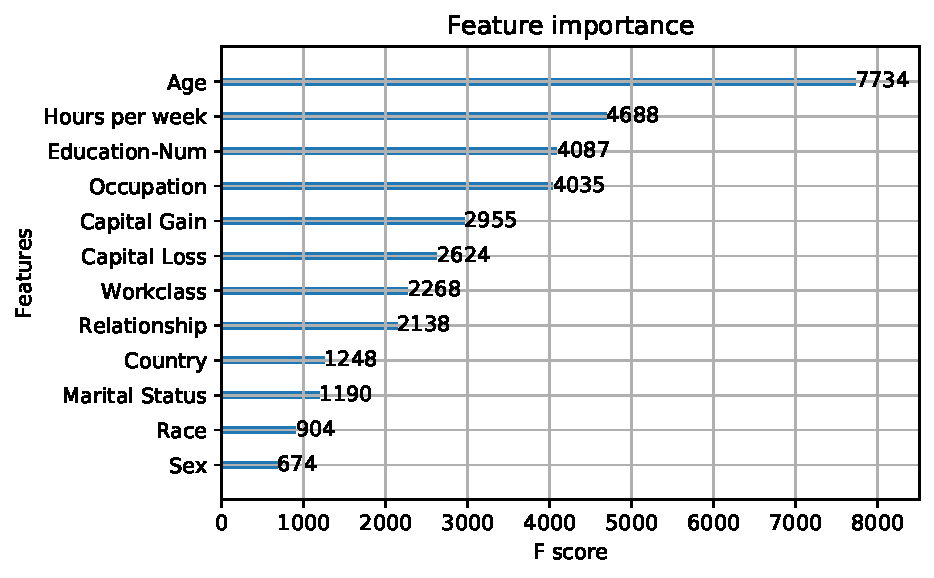
\includegraphics[scale=0.75]{figures/xgboost.plot.pdf}
	\caption{График важности признаков \lstinline{xgboost.plot_importance(model)},\\построенный с помощью пакета \texttt{xgboost} }\label{fig:xgboost_plot}
\end{figure}

\begin{figure}[h]
	\centering
	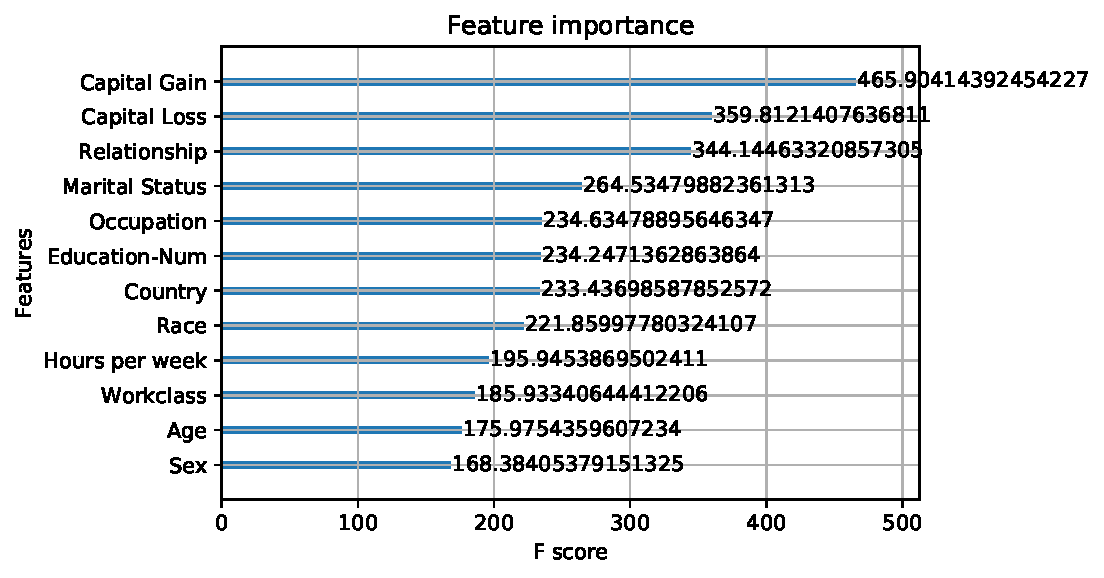
\includegraphics[scale=0.75]{figures/xgboost.plot.cover.pdf}
	\caption{График важности признаков \lstinline{xgboost.plot_importance(model, importance_type='cover')},\\построенный с помощью пакета \texttt{xgboost} }\label{fig:xgboost_plot_cover}
\end{figure}

\begin{figure}[h]
	\centering
	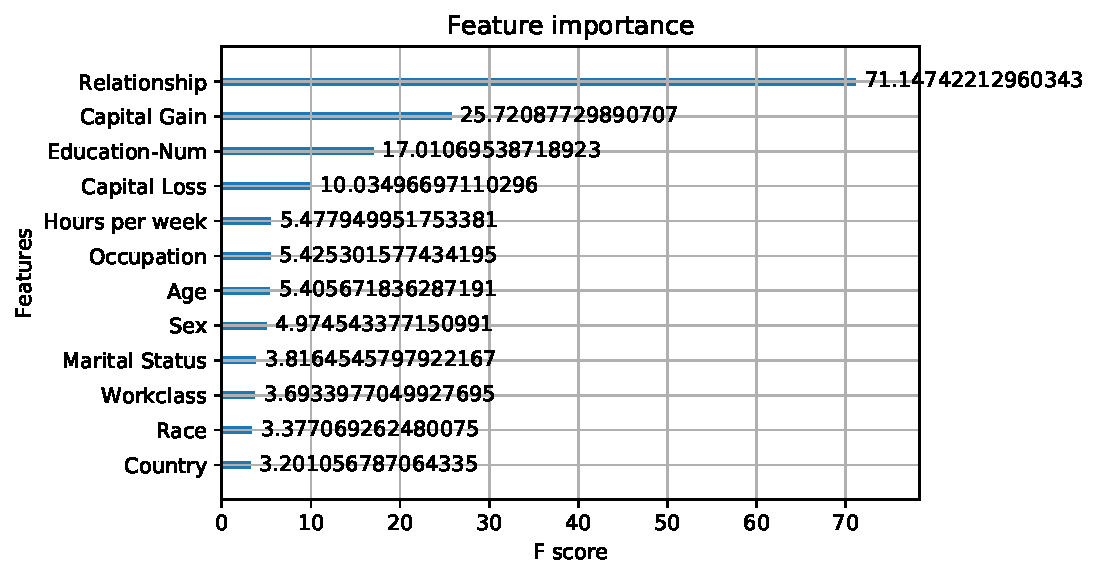
\includegraphics[scale=0.75]{figures/xgboost.plot.gain.pdf}
	\caption{График важности признаков \lstinline{xgboost.plot_importance(model, importance_type='gain')},\\построенный с помощью пакета \texttt{xgboost} }\label{fig:xgboost_plot_gain}
\end{figure}

Следует иметь в виду, что в библиотеке \texttt{xgboost} поддерживается три варианта вычисления важности признаков (см.~\href{https://towardsdatascience.com/interpretable-machine-learning-with-xgboost-9ec80d148d27}{Interpretable Machine Learning with XGBoost}):

\begin{itemize}
	\item \texttt{weight}: общее число сценариев по всем деревьям, когда $i$-ый признак используется для расщепления обучающего набора данных,
	
	\item \texttt{cover}: общее число сценариев по всем деревьям, когда $i$-ый признак используется для расщепления набора данных, взвешенное по числу точек обучающего набора данных, которые проходят через эти расщепления,
	
	\item \texttt{gain}: среднее снижение потерь на обучающем наборе данных, полученное при использовании $i$-ого признака.
\end{itemize}


\subsection{Особенности реализации в пакете \texttt{LightGBM}}

\subsection{Особенности реализации в пакете \texttt{CatBoost}}

\section{Форматирование строк в языке \texttt{Python}}

Пример форматирования строк в \texttt{Python} 

\begin{lstlisting}[
style = ironpython,
numbers = none
]
'{:*>+12.3f}, {:#^+17.5G}, {!r}'.format(
                                     math.pi,
                                     -math.exp(1)*10**(+6),
                                     type(list)  # для этого объекта будет
                                                 # использована функция repr()
                                 )
# "******+3.142, ###-2.7183E+06###, <class 'type'>"
\end{lstlisting}

Часть, стоящая после двоеточия, называется \emph{спецификатором формата} \cite[\strbook{283}]{ramalho:python-2016}. Полезные приемы форматирования можно найти в \cite{prohorenok:python-2016}.

\section{Хэшируемые пользовательские классы в языке \texttt{Python}}

Чтобы класс был хэшируемым, следует реализовать метод \texttt{\_\_hash\_\_}. Нужно также, чтобы векторы были \emph{неизменяемыми}. И этого можно добиться, сделав компоненты \texttt{x} и \texttt{y} свойствами, доступными только для чтения.

\begin{lstlisting}[
title = {\sffamily Пример неизменяемого, но нехэшируемого класса},
style = ironpython,
emph = {__init__, x, y, __iter__, __repr__, __str__, angle, __format__,
__bytes__, __eq__, __abs__, __bool__},
numbers = none
]
import array
import math

class Vector2d:
    '''
    Неизменяемый, но еще нехэшируемый класс
    '''
    typecode = 'd'

    def __init__(self, x, y):
        self.__x = x  # закрытый атрибут экземпляра класса
        self.__y = y  # закрытый атрибут экземпляра класса

    # открытое свойство; прочитать значение `x` можно, но нельзя передать новое значение
    @property  
    def x(self):
        return self.__x

    # открытое свойство; прочитать значение `y` можно, но нельзя передать новое значение
    @property  
    def y(self):
        return self.__y

    def __iter__(self):
        return (i for i in (self.x, self.y))

    def __repr__(self):
        class_name = type(self).__name__
        return '{}({!r}, {!r})'.format(class_name, *self)

    def __str__(self):
        return str(tuple(self))

    def angle(self):
        return math.atan2(self.y, self.x)

    def __format__(self, fmt_spec = ''):  # пользовательский формат
        if fmt_spec.endswith('p'):  # если спецификатор формата заканчивается на 'p',
                                    # то координаты выводятся в полярном формате
            fmt_spec = fmt_spec[:-1]
            coords = (abs(self), self.angle())
            outer_fmt = '<{}, {}>'
        else:
            coords = self
            outer_fmt = '({}, {})'
        components = (format(c, fmt_spec) for c in coords)
        return outer_fmt.format(*components)

    def __bytes__(self):
        return (bytes([ord(self.typecode)]) + bytes(array(self.typecode, self)))

    def __eq__(self, other):
        return tuple(self) == tuple(other)

    def __abs__(self):
        return math.hypot(self.x, self.y)

    def __bool__(self):
        return bool(abs(self))
\end{lstlisting}

То есть здесь декоратор \texttt{@property} помечает метод чтения свойств, который возвращает значение закрытого атрибута экземпляра класса \texttt{self.\_\_x} и \texttt{self.\_\_y}.

Так как в реализации класса есть метод \texttt{\_\_format\_\_}, можно печатать класс управляя форматом, например,

\begin{lstlisting}[
title = {\sffamily Пример использования класса с реализованным методом \texttt{\_\_format\_\_}},
style = ironpython,
numbers = none
]
>>> v1 = Vector2d(10, 5)
>>> '{:*^+12.3gp}'.format(v1)  # '<***+11.2****, ***+0.464***>'
>>> '{:.3f}'.format(v1)  # '(10.000, 5.000)'
\end{lstlisting}

Наконец, можно реализовать метод \texttt{\_\_hash\_\_}. Он должен возвращать \texttt{int} и в идеале учитывать хэши объектов-атрибутов, потому что у равных объектов хэши также должны быть одинаковыми.

В документации по специальному методу \texttt{\_\_hash\_\_} рекомендуется объединять хэши компонентов с помощью побитового оператора\footnote{Побитовые операторы рассматривают операнды как бинарные последовательности} \emph{исключающего ИЛИ} (\texttt{\^}) \cite[\strbook{287}]{ramalho:python-2016}

\begin{lstlisting}[
style = ironpython,
emph = {__hash__},
numbers = none
]
...
def __hash__(self):
    return hash(self.__x) ^ hash(self.__y)  # побитовое исключающее ИЛИ
\end{lstlisting}

Теперь класс \texttt{Vector2d} стал \emph{хэшируемым}.

\begin{lstlisting}[
style = ironpython,
numbers = none
]
>>> v1 = Vector2d(3, 4)
>>> v2 = Vector2d(3.1, 4.2)
>>> hash(v1), hash(v2)  # (7, 384307168202284039)
>>> set([v1, v2])  # {Vector2d(3, 4), Vector2d(3.1, 4.2)}
\end{lstlisting}

\remark{
Строго говоря, для создания хэшируемого типа необязательно вводить свойства или как-то иначе защищать атрибуты экземпляра класса от изменения. Требуется только корректно реализовать методы \texttt{\_\_hash\_\_} и \texttt{\_\_eq\_\_}. Но хэш-значения экземпляра никогда не должно изменяться \cite[\strbook{288}]{ramalho:python-2016}
}

 
\section{Области видимости в языке \texttt{Python}}

Когда мы говорим о поиске значения имени применительно к программному коду, под термином \emph{область видимости} подразумевается \emph{пространство имен} -- то есть место в программном коде, где имени было присвоено значение \cite{lutz:learningpython-2011}.

В любом случае область видимости переменной (где она может использоваться) всегда определяется местом, где ей было присвоено значение.

\remark{%
Термины <<\emph{область видимости}>> и <<\emph{пространство имен}>> можно использовать как синонимичные
}

При каждом вызове функции создается новое \emph{локальное пространство имен}. Это пространство имен представляет локальное окружение, содержащее имена параметров функции, а также имена переменных, которым были присвоены значения в теле функции.

По умолчанию операция присваивания создает локальные имена (это поведение можно изменить с помощью \texttt{global} или \texttt{local}).

Схема разрешения имен в языке \texttt{Python} иногда называется \emph{правилом LEGB}\footnote{Local, Enclosing, Global, Built-in} \cite[\strbook{477}]{lutz:learningpython-2011}:

\begin{itemize}
	\item Когда внутри функции выполняется обращение к неизвестному имени, интерпретатор пытается отыскать его в четырех областях видимости -- в \emph{локальной}, затем в \emph{локальной области любой объемлющей функции} или в выражении \texttt{lambda}, затем в \emph{глобальной} и, наконец, во \emph{встроенной}. Поиск завершается, как только будет найдено первое подходящее имя.
	
	\item Когда внутри функции выполняется операция присваивания \lstinline{a=10} (а не обращения к имени внутри выражения), интерпретатор всегда создает или изменяет имя в \emph{локальной области видимости}, если в этой функции оно не было объявлено глобальным или нелокальным.
\end{itemize}

Пример

\begin{lstlisting}[
style = ironpython,
numbers = none
]
# глобальная область видимости
X = 99  

def func(Y):  # Y и Z локальные переменные
    # локальная область видимости
    Z = X + Y # X - глобальная переменная
    return Z
    
func(1)  # Y = 1
\end{lstlisting}

Переменные \texttt{Y} и \texttt{Z} являются \emph{локальными} (и существуют только во время выполнения функции), потому что присваивание значений обоим именам осуществляется внутри определения функции: присваивание переменной \texttt{Z} производится с помощью инструкции \texttt{=}, а \texttt{Y} -- потому что аргументы всегда передаются через операцию присваивания.

Когда внутри функции выполняется операция присваивания значения переменной, она всегда выполняется в \emph{локальном пространстве имен функции}

\begin{lstlisting}[
style = ironpython,
emph = {f},
numbers = none
]
a = 10  # глобальная область видимости

def f():
    a = 100  # локальная область видимости
    return a
\end{lstlisting}

В результате переменная \texttt{a} в теле функции ссылается на совершенно другой объект, содержащий значение 100, а не тот, на который ссылается внешняя переменная.

Переменные во вложенных функциях привязаны к \emph{лексической области видимости}. То есть поиск имени переменной начинается в \emph{локальной области видимости} и затем последовательно продолжается во всех \emph{объемлющих областях видимости внешних функций}, в направлении от внутренних к внешним.

Если и в этих \emph{пространствах имен} искомое имя не будет найдено, поиск будет продолжен в \emph{глобальном пространстве имен}, а затем во \emph{встроенном пространстве имен}, как и прежде.

При обращении к локальной переменной до того, как ей будет присвоено значение, возбуждается исключение \texttt{UnboundLocalError}. Следующий пример демонстрирует один из возможных сценариев, когда такое исключение может возникнуть

\begin{lstlisting}[
style = ironpython,
emph = {foo},
numbers = none
]
i = 0
def foo():
    i = i + 1  # приведет к исключению UnboundLocalError
    print(i)
\end{lstlisting}

В этой функции переменная \texttt{i} определяется как \emph{локальная} (потому что внутри функции ей присваивается некоторое значение и отсутствует инструкция \texttt{global}).

При этом инструкция присваивания \lstinline{i = i + 1} пытается прочитать значение переменной \texttt{i} еще до того, как ей будет присвоено значение.

Хотя в этом примере существует глобальная переменная \texttt{i}, она не используется для получения значения. Переменные в функциях могут быть либо \emph{локальными}, либо \emph{глобальными} и не могут произвольно изменять \emph{область видимости} в середине функции.

\remark{
Оператор \texttt{global} делает локальную переменную в теле функции \emph{глобальной} и говорит интерпретатору чтобы тот не искал переменную в локальной области видимости текущей функции
}

Например, нельзя считать, что переменная \texttt{i} в выражении \lstinline{i + 1} в предыдущем фрагменте обращается к глобальной переменной \texttt{i}; при этом переменная \texttt{i} в вызове \texttt{print(i)} подразумевает локальную переменную \texttt{i}, созданную в предыдущей инструкции.

\quinta{%
	Когда интерпретатор, построчно сканируя тело функции \texttt{def}, натыкается на строку \texttt{i = i + 1}, он заключает что переменная \texttt{i} является \emph{локальной}, так как ей присваивается значение именно в теле функции. А когда функция вызывается на выполнение и интерпретатор снова доходит до строки \texttt{i = i + 1}, выясняется, что переменная \texttt{i}, стоящая в правой части, не имет ссылок на какой-либо объект и потому возникает ошибка \texttt{UnboundLocalError}
}

\section{Декораторы в \texttt{Python}}

\emph{Декораторы} выполняются \emph{сразу после} загрузки или импорта модуля, однако увидеть какие-либо изменения можно только в том случае, если декоратор явно взаимодействует с пользователем на <<верхнем уровне>>\footnote{Если декоратор простой одноуровневый, то под верхним уровнем понимается его локальная область видимости, а если декоратор содержит замыкание, то -- понимается область видимости объемлющей функции}, например, печатает строку в терминале.  \emph{Задекорированные} же { функции} выполняются строго в результате явного вызова \cite[\strbook{217}]{ramalho:python-2016}.

\subsection{Реализация простого декоратора}

Рассмотрим простой декоратор, который хронометритует каждый вызов задекорированной функции и печатает затраченное время

\begin{lstlisting}[
style = ironpython,
title = {\sffamily clockdeco.py, не очень удачный пример декоратора},
emph = {clock, clocked},
numbers = none
]
import time

def clock(func):
    print('test string from `clock`')  # <- строка будет выведена в терминал
                                       # сразу после загрузки модуля, который
                                       # импортирует данный декоратор
    def clocked(*args):  # замыкание
        t0 = time.perf_counter()  # запомнить начальный момент времени
        result = func(*args)  # вызвать функцию
        elapsed = time.perf_counter() - t0  # вычислить сколько прошло времени
        name = func.__name__
        arg_str = ', '.join(repr(arg) for arg in args)
        print(f'{elapsed}, {name}({arg_str}) -> {result}')
        return result  # вернуть результат
return clocked
\end{lstlisting}

Использование декоратора выглядит так

\begin{lstlisting}[
label = {lst:deco},
style = ironpython,
title = {\sffamily clockdeco\_demo.py},
emph = {simple_deco_1, simple_deco_2,
simple_func_1, simple_func_2, inner, snooze, factorial}
]
import time
from clockdeco import clock

def simple_deco_1(f): 
    '''
    Декоратор с замыканием
    '''
    def inner():
        print('test string from `simple_deco_1`')  # <- строка НЕ будет выведена
                                                   # после загрузке модуля
    return inner

def simple_deco_2(f):
    '''
    Простой одноуровневый декоратор
    '''
    print('test string from `simple_deco_2`')  # <- строка будет выведена в терминал
                                               # сразу после загрузки модуля
    return f

@simple_deco_1  # simple_func_1 = simple_deco_1(f=simple_func_1) -> inner
def simple_func_1():
    print('test string from `simple_func_1`')   

@simple_deco_2  # simple_func_2 = simple_deco_2(f=simple_func_2) -> simple_func_2
def simple_func_2():
    print('test string from `simple_func_2`')   

@clock  # snooze = clock(func=snooze) -> clocked
def snooze(seconds):
    time.sleep(seconds)

@clock
def factorial(n):
    return 1 if n < 2 else n*factorial(n-1)


if __name__ == '__main__':
    print('*'*10, 'Calling snooze(.123)')
    print('snooze_result = {}'.format(snooze(.123)))
    print('*'*10, 'Calling factorial(6)')
    print('6! = ', factorial(6))
    print(f'This is result from `simple_func_1`: {simple_func_1()}')
    print(f'This is result from `simple_func_2`: {simple_func_2()}')
\end{lstlisting}

\begin{lstlisting}[
title = {\sffamily Вывод clockdeco\_demo.py},
numbers = none
]
test string from `simple_deco_2`
test string from `clock`
test string from `clock`
********** Calling snooze(.123)
0.1261, snooze(0.123) -> None
snooze_result = None
********** Calling factorial(6)
1.866e-06, factorial(1) -> 1
7.589e-05, factorial(2) -> 2
0.0001266, factorial(3) -> 6
0.0001732, factorial(4) -> 24
0.0002224, factorial(5) -> 120
0.0002715, factorial(6) -> 720
6! =  720
test string from `simple_deco_1`
this is result from `simple_func_1`: None
test string from `simple_func_2`
this is result from `simple_func_2`: None
\end{lstlisting}

\remark{
Приведенный выше пример декоратора \texttt{clock} из модуля \texttt{clockdeco.py} не удачен в том смысле, что если нам, например, потребуется вывести значение атрибута \texttt{\_\_name\_\_} задекорированной функции \texttt{snooze}, т.е. \texttt{snooze.\_\_name\_\_}, то будет возвращена строка \texttt{'clocked'}, а не \texttt{'snooze'}.

Чтобы декоратор <<не портил>> значения атрибута \texttt{\_\_name\_\_}, следует задекорировать замыкание декоратора с помощью \texttt{@functools.wraps(func)}
}


При разгрузке модуля \texttt{clockdeco\_demo.py} будут выполнены все декораторы, но только декораторы \texttt{simple\_deco\_2} и \texttt{clock} выведут в терминал строки, потому как эти строки расположены на верхнем уровне декораторов (т.е. находятся не внутри вложенных функций). Декоратор \texttt{simple\_deco\_1} ничего не выводит, так как строка находится в области видимости вложенной функции.

Важно отметить следующее: после загрузки модуля, как уже говорилось выше, будут выведены в терминал строки, расположенные на верхнем уровне декораторов, но самое главное заключается в том, что после выполнения декоратора \texttt{clock} объект \texttt{snooze} уже будет ссылаться на внутреннюю функцию \texttt{clocked} декоратора \texttt{clock}, а после выполнения декоратора \texttt{simple\_deco\_1} объект \texttt{simple\_func\_1} будет ссылаться на внутреннюю функцию \texttt{inner}. Что же касается декоратора \texttt{simple\_deco\_2}, то объект \texttt{simple\_func\_2} будет ссылаться на \texttt{simple\_func\_2}.

По этой причине при вызове функции \texttt{simple\_func\_1()} печатается строка из внутренней функции \texttt{inner}, а при вызове функции \texttt{simple\_func\_2()} -- строка из этой же функции.

Еще один пример декоратора с замыканием

\begin{lstlisting}[
style = ironpython,
emph = {deco, inner, target},
numbers = none
]
def deco(f):
    def inner(*args, **kwargs):
        print(f'from `deco-inner`: args={args}, kwargs={kwargs}')
        return f  # f - свободная переменная
    return inner

@deco  # target = deco(f=target) -> inner :: target -> inner :: target=inner
def target(a, b=10):
    return (f'from `target`: a={a}, b={b}')

print(target(20, b=500)(250))  # сначала вызывается inner(20, b=500), а потом target(250)
\end{lstlisting}

Выведет

\begin{lstlisting}[
numbers = none
]
from `deco-inner`: args=(20,), kwargs={'b': 500}
from `target`: a=250, b=10
\end{lstlisting}

\subsection{Кэширование с помощью \texttt{functools.lru\_cache}}

Декоратор \texttt{functools.lru\_cache} очень полезен на практике. Он реализует запоминание: прием оптимизации, смысл которого заключается в сохранении результатов предыдущих дорогостоящих вызовов функции, что позволяет избежать повторного вычисления с теми же аргументами, что и раньше \cite[\strbook{230}]{ramalho:python-2016}.

Например

\begin{lstlisting}[
style = ironpython,
emph = {fibonacci},
numbers = none
]
import functools
from clockdeco import clock

@functools.lru_cache
@clock
def fibonacci(n):
    if n < 2:
        return n
    return fibonacci(n-2) + fibonacci(n-1)
    
if __name__ == '__main__':
    print(fibonacci(6))
\end{lstlisting}

\remark{
\texttt{lru\_cache} хранит результаты в словаре, ключи которого составлены из позиционных и именованных аргументов вызовов, а это значит, что все аргументы, принимаемые декорируемой функции должны быть \emph{хешируемыми}
}

\subsection{Одиночная диспетчеризация и обобщенные функции}

Декоратор \texttt{functools.singledispatch} позволяет каждому модулю вносить свой вклад в общее решение. Обычная функция, декорированная \texttt{@singledispatch} становится \emph{обобщенной функцией}: групповой функцией, выполняющей одну и ту же логическую операцию по-разному в зависимости от типа первого аргумента \cite[\strbook{234}]{ramalho:python-2016}. Именно это и называется \emph{одиночной диспетчеризацией}. Если бы для выбора конкретных функций использовалось больше аргументов, то мы имели бы дело с \emph{множественной диспетчеризацией}.

Например

\begin{lstlisting}[
style = ironpython,
emph = {htmlize},
numbers = none
]
from functools import singledispatch
from collections import abc
import numbers
import html

@singledispatch  # делает функцию обобщенной
def htmlize(obj):
    content = html.escape(repr(obj))
    return '<pre>{}</pre>'.format(content)
    
    
@htmlize.register(str)  # будет вызываться для объектов строкового типа данных
def _(text):
    content = html.escape(text).replace('\n', '<br>\n')
    return '<p>{}</p>'.format(content)
    
    
@htmlize.register(numbers.Integral)  # будет вызваться для объектов целочисленного типа данных
def _(n):
    return '<pre>{} (0x{:x})</pre>'.format(n)
    
    
@htmlize.register(tuple)
@htmlize.register(abc.MutableSequence)
def _(seq):
    inner = '</li>\n<li>'.join(htmlize(item) for item in seq)
    return '<ul>\n<li>' + inner + '</li>\n</ul>'
\end{lstlisting}

\remark{
По возможности следует стараться регистрировать специализированные функции для обработки абстрактных базовых классов, например, \texttt{numbers.Integral} или \texttt{abc.MutableSequence}, а не конкретные реализации типа \texttt{int} или \texttt{list}
}

Замечательное свойство механизма \texttt{singledispatch} состоит в том, что специализированные функции можно зарегистрировать в любом месте системы, в любом модуле \cite{ramalho:python-2016}.

\subsection{Композиции декораторов}

Когда два декоратора \texttt{@d1} и \texttt{@d2} применяются к одной и той же функции \texttt{f} в указанном порядке, получается то же самое, что в результате композиции \texttt{f = d1(d2(f))}.

Иными словами

\begin{lstlisting}[
style = ironpython,
emph = {f},
numbers = none
]
@d1
@d2
def f():
    print('f')
\end{lstlisting}
эквивалентен следующему
\begin{lstlisting}[
style = ironpython,
emph = {f},
numbers = none
]
def f():
    print('f')
    
f = d1(d2(f))
\end{lstlisting}

Рассмотрим еще один пример композиции декораторов

\begin{lstlisting}[
style = ironpython,
emph = {deco1, deco2, target, inner1, inner2},
numbers = none
]
def deco1(f):  # выполняется вторым
    print('deco-1')  # # будет выведена в терминал
    def inner1():
        print('string from `deco1-inner`')
    return inner1

def deco2(f):  # выполняется первым
    print('deco-2')  # будет выведена в терминал
    def inner2():
        print('string from `deco2-inner')
    return inner2

@deco1  # 2) inner2 = deco1(f=inner2) -> inner1 :: inner2 -> inner1 :: inner2 = inner1
@deco2  # 1) target = deco2(f=target) -> inner2 :: target -> inner2 :: target = inner2
def target():  # 3) target -> inner1
    print('string from `target`')


if __name__ == '__main__':
    target()  # выведет string from `deco1-inner`
\end{lstlisting}

Выведет

\begin{lstlisting}[
numbers = none
]
deco-2
deco-1
string from `deco1-inner`
\end{lstlisting}

\remark{
Первым выполняется тот декоратор, который ближе расположен к декорируемой функции
}


То есть при загрузке или импорте модуля будут выполнены декораторы \texttt{deco1} и \texttt{deco2}: сначала \texttt{deco2}, а затем \texttt{deco1}, потому как \texttt{deco2} ближе к декорируемой функции. Декоратор \texttt{deco1} применяется к той функции, которую возвращает \texttt{deco2}.

\subsection{Параметризованные декораторы}

Параметризованные декораторы часто называют \emph{фабриками декораторов}. Фабрики декораторов возвращают настоящие декораторы, которые применяются к декорируемой функции.

Пример

\begin{lstlisting}[
style = ironpython,
emph = {register, decorate, f1, f2, f3},
numbers = none
]
registry = set()

def register(activate=True):  # фабрика декораторов
    def decorate(func):  # декоратор
        print(f'running register(activate={activate})->decorate({func})')
        if activate:
            registry.add(func)
        else:
            registry.discard(func)
        return func
    return decorate

@register(activate=False)  # f1 = decorate(func=f1) -> f1 :: f1 -> f1
def f1():
    print('running f1()')

@register()  # f2 = decorate(func=f2) -> f2 :: f2 -> f2
def f2():
    print('running f2()')

def f3():
print('running f3()')
\end{lstlisting}

Идея в том, что функция \texttt{register()} возвращает декоратор \texttt{decorate}, который затем применяется к декорируемой функции \cite{ramalho:python-2016}. 

\remark{
\emph{Фабрика декораторов} возвращает \emph{декоратор}, который применяется к декорируемой функции
}

Чуть подробнее: сразу после загрузки или импорта модуля выполняется фабрика декораторов \texttt{register}, которая возвращает декоратор \texttt{decorate}, который и применяется к функциям. Можно представлять, что фабрика декораторов нужна только для того, чтобы собрать значения каких-то дополнительных переменных, которые потребуются позже. В данном примере можно представить, что строка \texttt{@register()} заменяется на строку \texttt{@decorate}. То есть декоратор применяется к функции, расположенной на следующей строке, и работает как обычно.

Как можно работать с этой фабрикой декораторов

\begin{lstlisting}[
style = ironpython,
numbers = none
]
register()(f3)  # добавить ссылку на функцию f3 во множенство registry
register(activate=False)(f2)  # удалить ссылку на функцию f2
\end{lstlisting}

Конструкция \texttt{register()} возвращает декоратор, который затем применяется к переменной (например, к \texttt{f3}), ассоциированной с декорируемой функцией, и работает так, как если бы изначально был только он (без фабрики декораторов) \cite{ramalho:python-2016}.

Если бы у декоратора был еще один уровень вложенности, т.е. было бы определено еще и замыкание, то это изменило бы только ссылку на функцию, которую возвращает замыкание

\begin{lstlisting}[
style = ironpython,
emph = {fabricdeco, deco, inner, target},
numbers = none
]
def fabricdeco():  # фабрика декораторов
    def deco(f):  # декоратор
        def inner():  # замыкание
            print(f'from inner: {f}')
        return inner
    return deco
    
@fabicdeco()  # target = deco(f=target) -> inner :: target -> inner :: target=inner
def target():
    print('from target')
    
target()  # на самом деле вызывается inner() -> from inner: <function target at 0x0...08B05318>
\end{lstlisting}

Рассмотрим еще один пример параметризованного декоратора

\begin{lstlisting}[
style = ironpython,
emph = {clock, clocked, decorate, snooze},
numbers = none
]
import time

DEFAULT_FMT = '[{elapsed}s] {name}({args}) -> {result}'

def clock(fmt=DEFAULT_FMT):  # фабрика декораторов
    def decorate(func):  # декоратор
        count = 0
        def clocked(*_args):  # замыкание
            nonlocal count  # делает переменную свободной
            count += 1
            print(f'args-{count}: {_args}')
            t0 = time.time()
            _result = func(*_args)
            elapsed = time.time() - t0
            name = func.__name__
            args = ', '.join(repr(arg) for arg in _args)
            result = repr(_result)
            print(fmt.format(**locals())) # использование **locals() позволяет ссылаться
                                          # на любую локальную переменную clocked
            return _result
        return clocked
    return decorate


if __name__ == '__main__':
    @clock()  # snooze = decorate(func=snooze) -> clocked :: snooze -> clocked
    def snooze(seconds):
        time.sleep(seconds)

    for i in range(3):
        snooze(0.123)
\end{lstlisting}

Теперь фабрику декораторов можно вызывать, например, так:
\begin{lstlisting}[
style = ironpython,
emph = {snooze},
numbers = none
]
@clock('log::{name}({args}), dt={elapsed:.5g}s')
def snooze(seconds):
    time.sleep(seconds)
\end{lstlisting}

Объяснение: сразу после загрузки модуля (когда модуль загружается как скрипт), интерпретатор наталкивается на строку \texttt{@clock()} после чего вызывает \emph{фабрику декораторов} \texttt{clock}, которая возвращает ссылку на \emph{декоратор} \texttt{decorate}, который в свою очередь начинает работать как и в описанных выше случаях, т.е. аргумент \texttt{func} декоратора получает ссылку на \texttt{snooze}, а сам декоратор возвращает ссылку на \emph{замыкание} \texttt{clocked}.

\remark{
Интерпретатор вызывает декоратор или фабрику декораторов из той строки, в которой находится конструкция \texttt{@deco}, поэтому как в данном примере если \texttt{@clock()} разместить в блоке проверки значения атрибута \texttt{\_\_name\_\_}, то фабрика декораторов не будет вызвана
}

Однако здесь есть любопытный момент. Переменные \texttt{func} и \texttt{count} вообще говоря являются \emph{свободными переменными}, поэтому их значения можно читать из-под замыкания (находясь в области видимости замыкания) даже после того, как локальная область видимости объемлющей функции (декоратора) будет уничтожена. Но если попытаться передать новое значение переменной \texttt{count}, находясь в теле замыкания \emph{без} использования оператора \texttt{nonlocal}, то это приведет к ошибке \texttt{UnboundLocalError}. Дело в том что свободные переменные по умолчанию можно только читать из-под замыкания. Когда мы присваиваем новое значение переменной \texttt{count} в теле замыкания, то мы делаем эту переменную локальной для замыкания \texttt{clocked}, переменная \texttt{count} перестает быть свободной. Чтобы объяснить интерпретатору, что переменная \texttt{count} должна рассматриваться как свободная даже если ей присваивается значение в области видимости замыкания, следует использовать оператор \texttt{nonlocal}.


\subsection{Обобщение по механизму работы декораторов}

Если обобщить сказанное выше, то получается, что задекорированная функция ссылается на ту функцию, которую возвращает декоратор, аргумент которого получил ссылку на данную функцию. И происходит это \emph{сразу после} загрузки или импорта модуля. А затем остается только вызвать задекорированную функцию, которая вообще говоря уже ссылается на какую-то другую функцию, которую возвращает декоратор, т.е. если
\begin{lstlisting}[
style = ironpython,
emph = {deco, inner, target},
numbers = none
]
def deco(f):
    def inner():  # замыкание
        print('inner')
    return inner
    
@deco  # выполняется при загрузке/импорте модуля
def target():
    print('target')
\end{lstlisting}
то
\lstinline[style = ironpython]{target = deco(f=target) -> inner}\\и, следовательно, \lstinline{target -> inner} (можно считать, что \lstinline{target=inner});\\поэтому при вызове \lstinline{target()} на самом деле вызывается \lstinline{inner()} и будет выведена строка \lstinline[style=ironpython]{'inner'} (см.~\pic{fig:target_deco_formula}).

\begin{figure}[h]
	\centering
	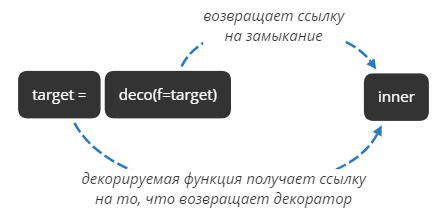
\includegraphics[scale=0.85]{figures/target_deco_formula.png}
	\caption{ К вопросу о механизме работы декоратора с вложенной функцией }\label{fig:target_deco_formula}
\end{figure}


\section{Замыкания/фабричные функции в \texttt{Python}}

Под термином \emph{замыкание} или \emph{фабричная функция} подразумевается объект функции, который сохраняет значения в \emph{объемлющих областях видимости}, даже когда эти области могут прекратить свое существование \cite[\strbook{488}]{lutz:learningpython-2011}.

В источнике \cite[\strbook{222}]{ramalho:python-2016} приводится несколько отличное определение\footnote{Определение содержит авторские правки}: \emph{замыкание} -- это вложенная функция с расширенной областью видимости, которая охватывает все \emph{неглобальные} переменные, объявленные в области видимости объемлющей функции, и способная работать с этими переменными даже после того как локальная область видимости объемлющей функции будет уничтожена.

Замыкания и вложенные функции особенно удобны, когда требуется реализовать концепцию отложенных вычислений \cite{beazley:python-2010}.

\remark{
Все же правильнее <<фабрикой функций>> называть всю конструкцию из объемлющей и вложенной функций, а <<замыканием>> -- только вложенную функцию
}

Рассмотрим в качестве примера следующую функцию

\begin{lstlisting}[
style = ironpython,
emph = {maker, action},
numbers = none
]
def maker(N):
    def action(X):
        return X**N  # функция action запоминает значение N в объемлющей области видимости
    return action
\end{lstlisting}

Здесь определяется внешняя функция, которая просто создает и возвращает вложенную функцию, не вызывая ее. Если вызвать внешнюю функцию

\begin{lstlisting}[
style = ironpython,
emph = {maker},
numbers = none
]
>>> f = maker(2)  # запишет 2 в N
>>> f  # <function action at 0x0147280>
\end{lstlisting}
она вернет ссылку на созданную ею вложенную функцию, созданную при выполнении вложенной инструкции \texttt{def}. Если теперь вызвать то, что было получено от внешней функции

\begin{lstlisting}[
style = ironpython,
numbers = none
]
>>> f(3)  # запишет 3 в X, в N по-прежнему хранится число 2
>>> f(4)  # 4**2
\end{lstlisting}
будет вызвана вложенная функция, с именем \texttt{action} внутри функции \texttt{maker}. Самое необычное здесь то, что вложенная функция продолжает хранить число 2, значение переменной \texttt{N} в функции \texttt{maker} даже при том, что к моменту вызова функции \texttt{action} функция \texttt{maker} уже \emph{завершила свою работу и вернула управление}.

Когда функция используется как вложенная, в замыкание включается все ее окружение, необходимое для работы внутренней функции \cite[\strbook{137}]{beazley:python-2010}.

\subsection{Области видимости и значения по умолчанию применительно к переменным цикла}

Существует одна известная особенность для функций или lambda-выражений: если lambda-выражение или инструкция \texttt{def} вложены в цикл внутри другой функции и вложенная функция ссылается на переменную из объемлющей области видимости, которая изменяется в цикле, все функции, созданные в этом цикле, будут иметь одно и то же значение -- значение, которое имела переменная на последней итерации \cite[\strbook{492}]{lutz:learningpython-2011}.

Например, ниже предпринята попытка создать список функций, каждая из которых запоминает текущее значение переменной \texttt{i} из объемлющей области видимости

\begin{lstlisting}[
title = {\sffamily Эта реализация работать НЕ будет},
style = ironpython,
emph = {makeActions},
numbers = none
]
def makeActions():
    acts = []
    for i in range(5):  # область видимости объемлющей функции
        acts.append(
            lambda x: i**x  # локальная область видимости вложенной анонимной функции
        ) 
    return acts
    
acts = makeActions()
print(acts[0](2))  # вернет 4**2, последнее значение i
print(acts[3](2))  # вернет 4**2, последнее значение i
\end{lstlisting}

Такой подход не дает желаемого результата, потому что поиск переменной в объемлющей области видимости производится позднее, \emph{при вызове вложенных функций}, в результате все они получат одно и то же значение (значение, которое имела переменная цикла на последней итерации).

Это один из случаев, когда необходимо явно сохранять значение из объемлющей области видимости в виде аргумента со значением по умолчанию вместо использования ссылки на переменную из объемлющей области видимости.

То есть, чтобы фрагмент заработал, необходимо передать текущее значение переменной из объемлющей области видимости в виде значения по умолчанию. Значения по умолчанию вычисляются в момент \emph{создания вложенной функции} (а не когда она \emph{вызывается}), поэтому каждая из них сохранит свое собственное значение \texttt{i}

\begin{lstlisting}[
title = {\sffamily Правильная реализация},
style = ironpython,
emph = {makeActions},
numbers = none
]
def makeActions():
    acts = []
    for i in range(5):
        acts.append(
            lambda x, i=i: i**x  # сохранить текущее значение i
        )
    return acts

acts = makeActions()
print(acts[0](2))  # вернет 0**2
print(acts[2](2))  # вернет 2**2
\end{lstlisting}

\quinta{%
Значения аргументов по умолчанию вложенных функций, динамически создаваемых в цикле на уровне области видимости объемлющей функции, вычисляются в момент \emph{создания} этих вложенных функций, а не в момент их вызова, поэтому \texttt{lambda x, i=i: ...} работает корректно
}

\section{Значения по умолчанию изменяемого типа данных в \texttt{Python}}

Если у функции есть аргумент, который получает ссылку на \emph{объект изменяемого типа данных} как на значение по умолчанию, то \emph{все вызовы функций} будут ссылаться на один и тот же изменяемый объект\footnote{По этой причине, как правило, только \emph{объекты неизменяемого типа данных} могут быть значениями по умолчанию. Если значение аргумента функции должно иметь возможность изменяться динамически, то этот аргумент функции инициализируют с помощью \texttt{None}, а затем передают ссылку на объект по условию} (идентификационный номер объекта не изменится).

Это удивляет. И когда говорят об аномальном поведении функции, аргумент которой ссылается на объект изменяемого типа данных, то обычно такое поведение объясняют следующим образом: значения аргументов по умолчанию вычисляются только один раз при загрузке модуля \cite[\strbook{77}]{slatkin:python-2016}. Однако такое объяснение не вскрывает механизм <<разделения>> ссылки между вызовами.

Лучше сказать так: если у функции есть аргумент, который ссылается на объект изменяемого типа данных, и в теле функции выполняется какая-то работа с этим изменяемым объектом (т.е. вносятся изменения в объект), то новые вызовы такой функции не сбрасывают значения по умолчанию до тех, которые были вычислены при загрузке модуля. Другими словами, если аргумент функции ссылается на объект изменяемого типа данных и над этим объектом выполняется какая-то работа в теле функции, то каждый новый вызов функции будет изменять этот изменяемый объект в \emph{определении} функции и потому каждый следующий вызов будет оперировать с уже измененным объектом изменяемого типа данных.

\remark{
Значения аргументов по умолчанию для избежания странного поведения функции должны ссылаться на \emph{объекты неизменяемого типа данных}
}

\section{Калибровка классификаторов}

Подробности в статье А. Дьяконова \href{https://dyakonov.org/2020/03/27/%D0%BF%D1%80%D0%BE%D0%B1%D0%BB%D0%B5%D0%BC%D0%B0-%D0%BA%D0%B0%D0%BB%D0%B8%D0%B1%D1%80%D0%BE%D0%B2%D0%BA%D0%B8-%D1%83%D0%B2%D0%B5%D1%80%D0%B5%D0%BD%D0%BD%D0%BE%D1%81%D1%82%D0%B8/}{<<Проблема калибровки уверенности>>}.
\vspace{2mm}

Ниже описываются способы оценить качество калибровки алгоритма. Надо сравнить \emph{уверенность} (confidence) и \emph{долю верных ответов} (accuracy) на тестовой выборке.

Если классификатор <<хорошо откалиброван>> и для большой группы объектов этот классификатор возвращает вероятность принадлежности к положительному классу 0.8, то среди этих объектов будет приблизительно 80\% объектов, которые в действительности принадлежат положительному классу. То есть, если для группы точек данных общим числом 100 классификатор возвращает вероятность положительного класса 0.8, то приблизительно 80 точек на самом деле будут принадлежать положительному классу и доля верных ответов тогда составит 0.8.

\subsection{Непараметрический метод гистограммной калибровки (Histogram Binning)}

Изначально в методе использовались бины одинаковой ширины, но можно использовать и равномощные бины.

Недостатки подхода:

\begin{itemize}
	\item число бинов задается наперед,
	
	\item функция деформации не непрерывна,
	
	\item в <<равноширинном варианте>> в некоторых бинах может содержаться недостаточное число точек.
\end{itemize}

Метод был предложен Zadrozny В. и Elkan C. \href{http://cseweb.ucsd.edu/~elkan/calibrated.pdf}{\ttfamily Obtaining  calibrated  probability  estimates  from  decision  trees  and naive bayesian classifiers}.

\subsection{Непараметрический метод изотонической регрессии (Isotonic Regression)}

Строится монотонно неубывающая функция деформации оценок алгоритма.

Метод был предложен Zadrozny B. и Elkan C. \href{http://citeseerx.ist.psu.edu/viewdoc/download?doi=10.1.1.13.7457&rep=rep1&type=pdf}{\ttfamily Transforming classifier scores into accurate multiclass probability estimates}.

Функция деформации по-прежнему не является непрерывной.

\subsection{Параметрическая калибровка Платта (Platt calibration)}

Изначально этот метод калибровки разрабатывался только для метода опорных векторов, оценки которого лежат на вещественной оси (по сути, это расстояния до оптимальной разделяющей классы прямой, взятые с нужным знаком). Считается, что этот метод не очень подходит для других моделей.

Предложен Platt~J. \href{http://citeseerx.ist.psu.edu/viewdoc/download;jsessionid=EA4888FEE74FB677B492740F59CDFE1F?doi=10.1.1.41.1639&rep=rep1&type=pdf}{\ttfamily Probabilistic  outputs  for  support  vector machines and comparisons to regularized likelihood methods}.

\subsection{Логистическая регрессия в пространстве логитов}

\subsection{Деревья калибровки}

Стандартный алгоритм строит строит суперпозицию дерева решений на исходных признаках и логистических регрессий (каждая в своем листе) над оценками алгоритма:

\begin{itemize}
	\item Построить на исходных признаках решающее дерево (не очень глубокое),
	
	\item В каждом листе -- обучить логистическую регрессию на одном признаке,
	
	\item Подрезать дерево, минимизируя ошибку.
\end{itemize}

\subsection{Температурное шкалирование (Temperature Scaling)}

Этот метод относится к классу DL-методов калибровки, так как он был разработан именно для калибровки нейронных сетей. Метод представляет собой простое многомерное обобщение шкалирования Платта.

\section{Приемы работы с менеджером пакетов \texttt{conda}}

\subsection{Создание виртуального окружения}

Создать виртуальное окружение \texttt{dashenv}

\begin{lstlisting}[
numbers = none
]
conda create --name dashenv
\end{lstlisting}

Создать виртуальное окружение с указанием версии \texttt{Python}

\begin{lstlisting}[
numbers = none
]
conda create --name testenv python=3.6
\end{lstlisting}

Создать виртуальное окружение с указанием пакета

\begin{lstlisting}[
numbers = none
]
conda create --name testenv scipy
\end{lstlisting}

Создать виртуальное окружение с указанием версии \texttt{Python} и нескольких пакетов

\begin{lstlisting}[
numbers = none
]
conda create --name testenv python=3.6 scipy=0.15.0 astroid babel
\end{lstlisting}

\remark{%
Рекомендуется устанавливать сразу несколько пакетов, чтобы избежать конфликта зависимостей
}

Для того чтобы при создании нового виртуального окружения не требовалось каждый раз устанавливать базовые пакеты, которые обычно используются в работе, можно привести их список в конфигурационном файле \texttt{.condarc} в разделе \texttt{create\_default\_packages}

\begin{lstlisting}[
title = {\sffamily .condarc},
numbers = none
]
ssl_verify: true
channels:
 - conda-forge
 - defaults
report_errors: true
default_python:
create_default_packages:
 - matplotlib
 - numpy
 - scipy
 - pandas
 - seaborn
\end{lstlisting}

Если для текущего виртуального окружения не требуется устанавливать пакеты из набора по умолчанию, то при создании виртуального окружения следует указать специальный флаг
\lstinline{--no-default-packages}

\begin{lstlisting}[
numbers = none
]
conda create --no-default-packages --name testenv python
\end{lstlisting}

Создать виртуальное окружение можно и из файла \texttt{environment.yml} (первая строка этого файла станет именем виртуального окружения)

\begin{lstlisting}[
title = {\sffamily environment.yml},
numbers = none
]
name: stats2
channels:
 - conda-forge
 - defaults
dependencies:
 - python=3.6   # or 2.7
 - bokeh=0.9.2
 - numpy=1.9.*
 - nodejs=0.10.*
 - flask
 - pip:
  - Flask-Testing
\end{lstlisting}

\begin{lstlisting}[
numbers = none
]
conda env create -f environment.yml
\end{lstlisting}

При создании виртуального окружения можно указать путь до целевой директории, где будут размещаться файлы окружения. Следующая команда создаст виртуальное окружение в поддиректории текущей рабочей директории \texttt{envs}\footnote{В данном случае чтобы удалить виртуальную среду достачно просто удалить директорию \texttt{envs}}

\begin{lstlisting}[
numbers = none
]
conda create --prefix ./envs jupyterlab matplotlib
\end{lstlisting}

С помощью файла спецификации можно создать \emph{идентичное виртуальное окружение} (i) на той же платформе операционной системы, (ii) на той же машине, (iii) на какой-либо другой машине (перенести настройки окружения).

Для этого предварительно требуется создать собственно файл спецификации

\begin{lstlisting}[
numbers = none
]
conda list --explicit > spec-file.txt
\end{lstlisting}

Имя файла спецификации может быть любым. Файл спецификации обычно не является кросс-платформенным и поэтому имеет комментарий в верхней части файла (\lstinline{#platform: osx-64}), указывающий платформу, на которой он был создан.

Теперь для того чтобы \emph{создать} окружение достаточно воспользоваться командой

\begin{lstlisting}[
numbers = none
]
conda create --name myenv --file spec-file.txt
\end{lstlisting}

Файл спецификации можно использовать для установки пакетов в существующее окружение

\begin{lstlisting}[
numbers = none
]
conda install --name myenv --file spec-file.txt
\end{lstlisting}


\subsection{Активация/деактивация виртуального окружения}

Активировать виртуальное окружение \texttt{dashenv}

\begin{lstlisting}[
numbers = none
]
conda activate dashenv
\end{lstlisting}

Активировать виртуальное окружение в случае, когда оно создавалось с \lstinline{--prefix}, можно указав полный путь до окружения
\begin{lstlisting}[
numbers = none
]
conda activate E:\[WorkDirectory]\[Python_projects]\directory_for_experiments\envs
\end{lstlisting}

В этом случае в строке приглашения командной оболочки по умолчанию будет отображаться полный путь до окружения. Чтобы заменить длинный префикс в имени окружения на более удобный псевдоним достаточно использовать конструкцию

\begin{lstlisting}[
numbers = none
]
conda config --set env_prompt ({name})
\end{lstlisting}
которая добавит в конфигурационный файл \texttt{.condarc} следующую строку

\begin{lstlisting}[
title = {\sffamily .condarc},
numbers = none
]
...
env_prompt: ({name})
\end{lstlisting}
и теперь имя окружения будет \texttt{(envs)}.

Деактивировать виртуальное окружение

\begin{lstlisting}[
numbers = none
]
conda deactivate
\end{lstlisting}

\subsection{Обновление виртуального окружения}

Обновить виртуальное окружение может потребоваться в следующих случаях:

\begin{itemize}
	\item обновилась одна из ключевых зависимостей,
	
	\item требуется добавить пакет (добавление зависимости),
	
	\item требуется добавить один пакет и удалить другой.
\end{itemize}

В любом из этих случаев все что нужно для того чтобы обновить виртуальное окружение это просто обновить файл \texttt{environment.yml}\footnote{Этот файл должен находится в той же директории что и директория окружения \texttt{envs}}, а затем запустить команду

\begin{lstlisting}[
numbers = none
]
conda env update --prefix ./envs --file environment.yml --prune
\end{lstlisting}

Опция \lstinline{--prune} приводит к тому, что \texttt{conda} удаляет все зависимости, которые больше не нужны для окружения.

\subsection{Вывод информации о виртуальном окружении}

Вывести список доступных виртуальных окружений

\begin{lstlisting}[
numbers = none
]
conda env list
\end{lstlisting}

Вывести список пакетов, установленных в указанном окружении

\begin{lstlisting}[
numbers = none
]
conda list --name myenv
\end{lstlisting}

Вывести информацию по конкретному пакету указанного окружения

\begin{lstlisting}[
numbers = none
]
conda list --name dashenv matplotlib
\end{lstlisting}


\subsection{Удаление виртуального окружения}

Удалить виртуальное окружение \texttt{heroku\_env}

\begin{lstlisting}[
numbers = none
]
conda env remove --name heroku_env
\end{lstlisting}

\subsection{Экспорт виртуального окружения в \texttt{environment.yml}}

Экспортировать активное виртуальное окружение в yml-файл

\begin{lstlisting}[
numbers = none
]
conda env export > environment.yml
\end{lstlisting}

\section{Приемы работы с пакетом \texttt{Vowpal Wabbit}}

\section{Приемы работы с библиотекой \texttt{pandas}}

\subsection{Число уникальных значений категориальных признаков в объекте \texttt{DataFrame}}

Для того чтобы вывести информацию по числу уникальных значений в каждом категориальном признаке некоторого объекта \texttt{pandas.DataFrame} можно воспользоваться конструкцией

\begin{lstlisting}[
style = ironpython,
numbers = none
]
X.select_dtypes('category').apply(lambda col: col.unique().shape[0])
\end{lstlisting}

\subsection{Число пропущенных значений в объекте \texttt{DataFrame}}

Информацию по числу пропущенных значений в каждом столбце можно вывести следующим образом

\begin{lstlisting}[
style = ironpython,
numbers = none
]
X.isna().any(axis=0)
\end{lstlisting}


\section{Интерпретация моделей и оценка важности признаков с библиотекой \texttt{SHAP}}

\subsection{Общие сведения о значениях Шепли}

В библиотеке \texttt{SHAP} \url{https://github.com/slundberg/shap} для оценки \emph{важности признаков} используются \emph{значения Шепли}\footnote{Термин пришел из теории кооперативных игр} (Shapley value) \url{https://en.wikipedia.org/wiki/Shapley_value}.

Или несколько точнее: при построении \emph{локальной} интерпретации (то есть интерпретации на конкретной точке данных) значения Шепли, строго говоря, оценивают \emph{силу влияния}\footnote{Еще эту оценку можно интерпретировать как \emph{вклад}} $ i $-ого признака $ f_i $ на значения целевого вектора $ y $, а вот \emph{важность признака} в контексте модели можно оценить при построении \emph{глобальной} интерпретации с помощью значений Шепли, взятых по абсолютной величине и усредненных по имеющемуся набору данных. 

\remark{
Значения Шепли объясняют как <<справедливо>> оценить вклад каждого признака в прогноз модели
}

Значения Шепли $i$-ого признака на \emph{конкретном объекте} (на текущей точке данных) вычисляются следующим образом (здесь сумма распространяется на все подмножества признаков $ S $ из множества признаков $ N $, не содержащие $ i $-ого признака)
\begin{align*}
\phi_i(v) = \sum_{S \subseteq N\setminus\{i\}} \dfrac{|S|!(n - |S| - 1)!}{n!}\Bigl( \underset{f_i-contribution }{\underbrace{ v(S \cup \{i\}) - v(S)}} \Bigr),
\end{align*}
где $ n $ -- общее число признаков; $ v(S \cup \{i\}) $ -- прогноз модели с учетом $ i $-ого признака; $ v(S) $ -- прогноз модели без $ i $-ого признака.

Выражение $ v(S \cup \{i\}) - v(S) $ -- это вклад $ i $-ого признака. Если теперь вычислить среднее вкладов по всем возможным перестановкам, то получится <<честная>> оценка вклада $ i $-ого признака.

Значение Шепли для $ i $-ого признака вычисляется для каждой точки данных (например, для каждого клиента в выборке) на всех возможных комбинациях признаков (в том числе и для пустых подмножеств $ S $).

\remark{
Метод анализа важности признаков, реализованный в библиотеке \texttt{SHAP}, является и \emph{согласованным}, и \emph{точным} (см. \href{https://towardsdatascience.com/interpretable-machine-learning-with-xgboost-9ec80d148d27}{Interpretable Machine Learning with XGBoost})
}



\subsection{ Пример построения локальной и глобальной интерпретаций }

Примеры использования библиотеки \texttt{SHAP} не только для tree-base моделей можно найти по адресу \url{https://github.com/slundberg/shap/tree/master/notebooks/tree_explainer}.

Решается задача регрессии для классического набора данных \texttt{boston}. Требуется предсказать стоимость квартиры. 

\begin{lstlisting}[
style = ironpython,
numbers = none
]
import shap
import os
import pandas as pd
import numpy as np
from pandas import DataFrame, Series
import matplotlib.pyplot as plt
from sklearn.ensemble import RandomForestRegressor, GradientBoostingRegressor
from sklearn.model_selection import train_test_split
from sklearn.datasets import load_boston
#%matplotlib inline  # если код оформляется в JupyterLab
#shap.initjs()  # если код оформляется в JupyterLab

boston = load_boston()
X, y = boston['data'], boston['target']  # numpy-массивы

# объекты pandas
X_full = DataFrame(X, columns=boston['feature_names'])
y_full = Series(y, name = 'PRICE')

X_train, X_test, y_train, y_test = train_test_split(X_full, y_full, random_state=42)

rf = RandomForestRegressor(n_estimators=500).fit(X_train, y_train)

explainer = shap.TreeExplainer(rf)  # <- NB
shap_values_train = explainer.shap_values(X_train)  # <- NB
\end{lstlisting}

\subsubsection{Локальная интерпретация отдельной точки данных обучающего набора}

Теперь можно построить локальную интерпретацию для одной точки данных из обучающего набора (см. \pic{fig:shap_force_plt_train})

\begin{lstlisting}[
style = ironpython,
title = {\sffamily К вопросу о локальной интерпретации отдельной точки данных обучающего набора},
numbers = none
]
row = 1
shap.force_plot(
    explainer.expected_value,  # ожидаемое значение
    shap_values_train[row, :],  # 2-ая строка в матрице значений Шепли
    X_train.iloc[row, :]  # 2-ая строка в обучающем наборе данных
)
\end{lstlisting}

Можно считать, что \texttt{explainer.expected\_value} это значение, полученное усреднением целевого вектора по точкам обучающего набора данных, т.е. \texttt{y\_train.mean()}.

\begin{figure}[h]
	\centering
	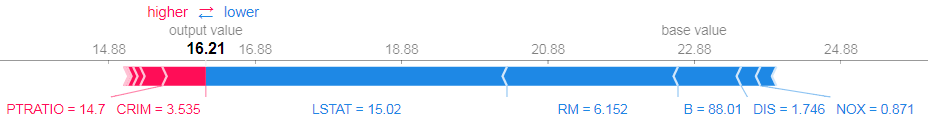
\includegraphics[scale=0.80]{figures/shap_force_plt_train.png}
	\caption{ Локальная интерпретация для одной точки данных обучающего набора }\label{fig:shap_force_plt_train}
\end{figure}

Еще можно построить график частичной зависимости (\pic{fig:shap_dependence_plt_train})

\begin{lstlisting}[
style = ironpython,
numbers = none
]
shap.dependence_plot('LSTAT', shap_values, X_train)
\end{lstlisting}

\begin{figure}[h]
	\centering
	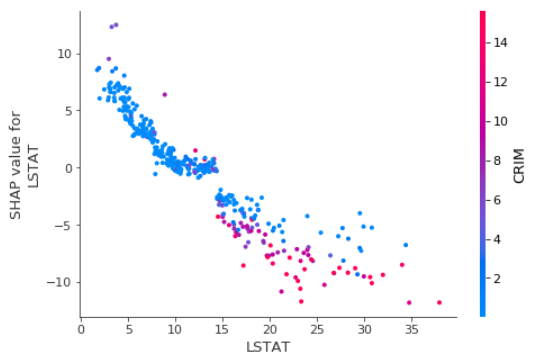
\includegraphics[scale=0.85]{figures/shap_dependence_plt_train.png}
	\caption{ График частичной зависимости признака \texttt{LSTAT} от значений Шепли\\с учетом влияния признака \texttt{CRIM} }\label{fig:shap_dependence_plt_train}
\end{figure}

\subsubsection{Локальная интерпретация отдельной точки данных тестового набора}

Прежде чем приступить к вычислению значений Шепли, следует создать поверхностную копию тестового набора данных

\begin{lstlisting}[
style = ironpython,
numbers = none
]
X_test_for_pred = X_test.copy()
X_test_for_pred['predict'] = np.round(rf.predict(X_test), 2)

explainer = shap.TreeExplainer(rf)
# вычисляем значения Шепли для тестового набора данных со столбцом 'predict'
shap_values_test = explainer.shap_values(X_test_for_pred)
\end{lstlisting}

Теперь можно построить локальную интерпретацию для отдельной точки данных тестового набора (\pic{fig:shap_dependence_plt_test}).

\begin{figure}
	\centering
	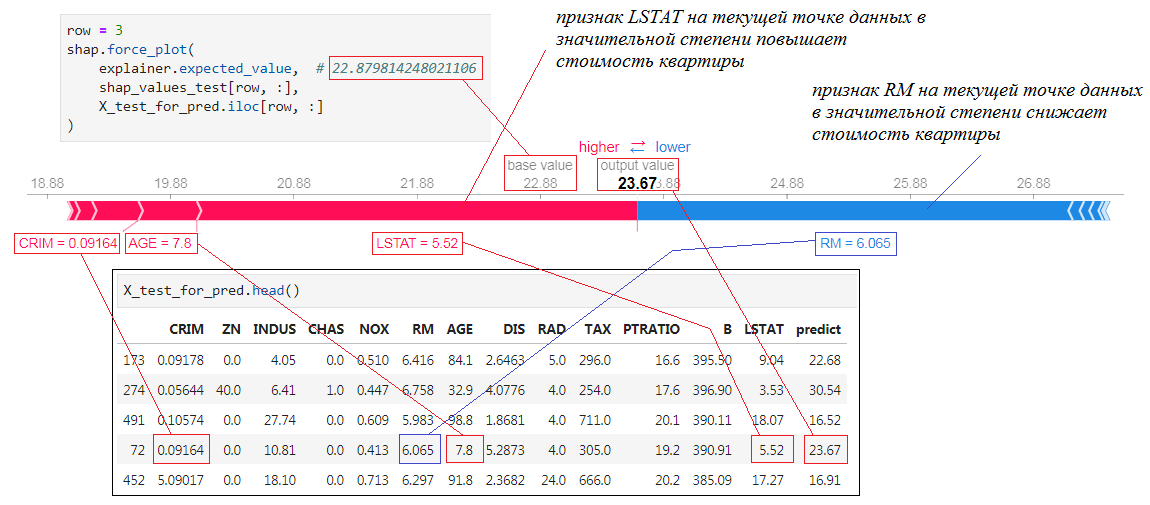
\includegraphics[scale=0.7]{figures/shap_dependence_plt_test.png}
	\caption{ Локальная интерпретация для одной точки данных тестового набора }\label{fig:shap_dependence_plt_test}
\end{figure}

Из \pic{fig:shap_dependence_plt_test} видно, что признаки с различной <<силой>>\footnote{Ширина полосы}, которая определяется значениями Шепли, смещают предсказание модели на данной точке. Например, признак \texttt{LSTAT} (процент населения с низким социальным статусом) в значительной степени \emph{повышает}\footnote{Потому что значение этого признака невелико; чем меньше процент населения с низким социальным статусом проживает в округе, тем выше стоимость квартиры} стоимость квартиры на \underline{данной точке} по отношению к базовому значению \texttt{base\_value}, а признак \texttt{RM} (среднее число комнат в жилом помещении) в значительной степени снижает.

\begin{lstlisting}[
style = ironpython,
title = {\sffamily К вопросу о локальной интерпретации отдельной точки данных тестового набора},
numbers = none
]
row = 3
shap.force_plot(
    explainer.expected_value,  # 22.879814248021106
    #y_train.mean()  # 22.907915567282323
    shap_values_test[row, :],
    X_test_for_pred.iloc[row, :]
)
\end{lstlisting}

\subsubsection{Глобальная интерпретация модели на тестовом наборе данных}

Удобно работать с диаграммой рассеяния \texttt{shap.summary\_plot} (\pic{fig:summary_plt_test}), на которой изображаются признаки в порядке убывания их важности, с одновременным указанием того, насколько сильно каждый из признаков влияет на целевую переменную.

\begin{lstlisting}[
style = ironpython,
numbers = none
]
shap.summary_plot(shap_values_test, X_test_for_pred)
\end{lstlisting}

\begin{figure}[h]
	\centering
	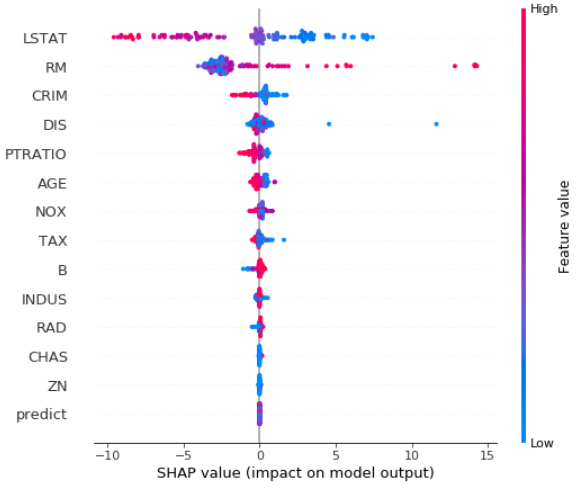
\includegraphics[scale=0.85]{figures/summary_plt_test.png}
	\caption{ Диаграмма рассеяния для точек тестового набора данных }\label{fig:summary_plt_test}
\end{figure}

Какие выводы можно сделать из \pic{fig:summary_plt_test}:

\begin{itemize}
	\item Признаки \texttt{LSTAT}, \texttt{RM} и \texttt{CRIM} имеют высокую важность для модели в целом,
	
	\item Для признака \texttt{LSTAT} наблюдается отрицательная статистическая зависимость от целевой переменной, т.е. низкие значения этого признака отвечают высоким значениям целевой переменной (стоимости на квартиру),
	
	\item Для признака \texttt{RM} наблюдается положительная статистическая зависимость от целевой переменной: чем больше комнат в жилом помещении, тем выше стоимость квартиры.
\end{itemize}

Затем можно детальнее изучить графики частичной зависимости, построенные на тестовом наборе данных. Рассмотрим зависимость признака \texttt{CRIM} (уровень преступности в городе на душу населения) от значений Шепли, вычисленных для этого признака (\pic{fig:dependeces_plt_test_CRIM}).

\begin{lstlisting}[
style = ironpython,
numbers = none
]
shap.dependence_plot('CRIM', shap_values_test[:, :-1], X_test_pred.iloc[:, :-1])
\end{lstlisting}

\begin{figure}[h!]
	\centering
	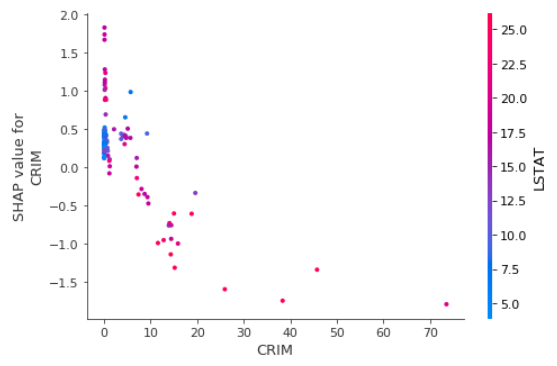
\includegraphics[scale=0.85]{figures/dependeces_plt_test_CRIM.png}
	\caption{ График частичной зависимости признака \texttt{CRIM} от значений Шепли\\с учетом влияния \texttt{LSTAT} }\label{fig:dependeces_plt_test_CRIM}
\end{figure}

Какие выводы можно сделать из \pic{fig:dependeces_plt_test_CRIM}:

\begin{itemize}
	\item Чем выше уровень преступности в городе, тем в большей степени снижается стоимость квартиры,
	
	\item Не везде, где проживает высокий процент населения с низким социальным статусом наблюдается высокий уровень преступности, однако в тех местах, где регистрируется высокий уровень преступности одновременно регистрируется и высокий процент населения с низким социальным статусом.
\end{itemize}


\section{Перестановочная важность признаков в библиотеке \texttt{eli5}}


Еще важность признаков можно оценивать с помощью так называемой \emph{перестановочной важности} (permutation importances) \url{https://www.kaggle.com/dansbecker/permutation-importance}.

Идея проста: нужно в заранее отведенном для исследования важности признаков наборе данных (валидационном наборе) перетасовать значения признака, влияние которого изучается на данной итерации, оставив остальные признаки (столбцы) и целевой вектор без изменения.

Признак считается <<важным>>, если метрики качества модели падают, и соответственно -- <<неважным>>, если перестановка не влияет на значения метрик. Перестановочная важность вычисляется после того как модель будет обучена.

\remark{
Перестановочная важность обладает свойством \emph{согласованности}, но не обладает свойством \emph{точности} \href{https://towardsdatascience.com/interpretable-machine-learning-with-xgboost-9ec80d148d27}{Interpretable Machine Learning with XGBoost}
}

Рассмотрим задачу построения регрессионной модели на наборе данных \texttt{load\_boston}

\begin{lstlisting}[
style = ironpython,
numbers = none
]
import eli5
import pandas as pd
from eli5.sklearn import PermutationImportance
from sklearn.ensemble import RandomForestRegressor
from sklearn.model_selection import train_test_split
from sklearn.datasets import load_boston
from pandas import DataFrame, Series

boston = load_boston()

X_train, X_test, y_train, y_test = train_test_split(boston['data'],
                                                    boston['target'], 
                                                    random_state=2)

X_train_sub, X_valid, y_train_sub, y_valid = train_test_split(X_train,
                                                              y_train,
                                                              random_state=0)

# модель случайного леса, как обычно, обучается на обучающей выборке
rf = RandomForestRegressor(n_estimators=500).fit(X_train_sub, y_train_sub)

# модель перестановочной важности обучается на валидационном наборе данных
perm = PermutationImportance(rf, random_state=42).fit(X_valid, y_valid)

eli5.show_weights(perm, feature_names = boston['feature_names'])  # визуализирует перестановочные важности признаков
\end{lstlisting}



% Источники в "Газовой промышленности" нумеруются по мере упоминания 
\begin{thebibliography}{99}\addcontentsline{toc}{section}{Список литературы}
	\bibitem{lutz:learningpython-2011}{{\emph{Лутц М.} Изучаем Python, 4-е издание. -- Пер. с англ. -- СПб.: Символ-Плюс, 2011. -- 1280~с. }
		
	\bibitem{beazley:python-2010}{\emph{Бизли Д.} Python. Подробный справочник. -- Пер. с англ. -- СПб.: Символ-Плюс, 2010. -- 864~с. }
	
	\bibitem{chacon:2020}{ \emph{Чакон С.}, \emph{Штрауб Б.} Git для профессионального программиста. -- СПб.: Питер, 2020. -- 496~с. }
	
	\bibitem{ramalho:python-2016}{\emph{Рамальо Л.}{ Python. К вершинам мастерства. -- М.: ДМК Пресс, 2016. -- 768 с.}}
	
	\bibitem{slatkin:python-2016}{ \emph{Слаткин  Б.} Секреты Python: 59 рекомендаций по написанию эффективного кода. -- М.: ООО~<<И.Д. Вильямс>>, 2016. -- 272~с.}
	
	\bibitem{prohorenok:python-2016}{ \emph{Прохоренок Н.А.}, \emph{Дронов В.А.} Python 3 и PyQt 5. Разработка приложений. -- СПб.: БХВ-Петербург, 2016. -- 832~с.}
\end{thebibliography}

%\listoffigures\addcontentsline{toc}{section}{Список иллюстраций}









\end{document}